\section{アルゴリズム(FAST)の概要}
私たちの班は,問題解決のアルゴリズムとしてFASTを用いた.
FASTの概要を以下に示す.

\subsection{原理}
FASTによる特徴量抽出の仕組みは以下のようなものである。
\begin{enumerate}
    \item あるピクセルにおける輝度値を$I_p$とする.
    \item 適当な閾値$t$を選ぶ.
    \item 周囲の16ピクセルに置いて,その輝度値が$I_p-t$より小さいか,$I_p+t$より大きいか,そのどちらでもないかを判定する.
    輝度値が$I_p-t$より小さいピクセルか,$I_p+t$より大きいピクセルがある数$n$以上の場合,その点を特徴点(corner)として抽出する.
\end{enumerate}
\begin{figure}[H]
    \begin{center}
        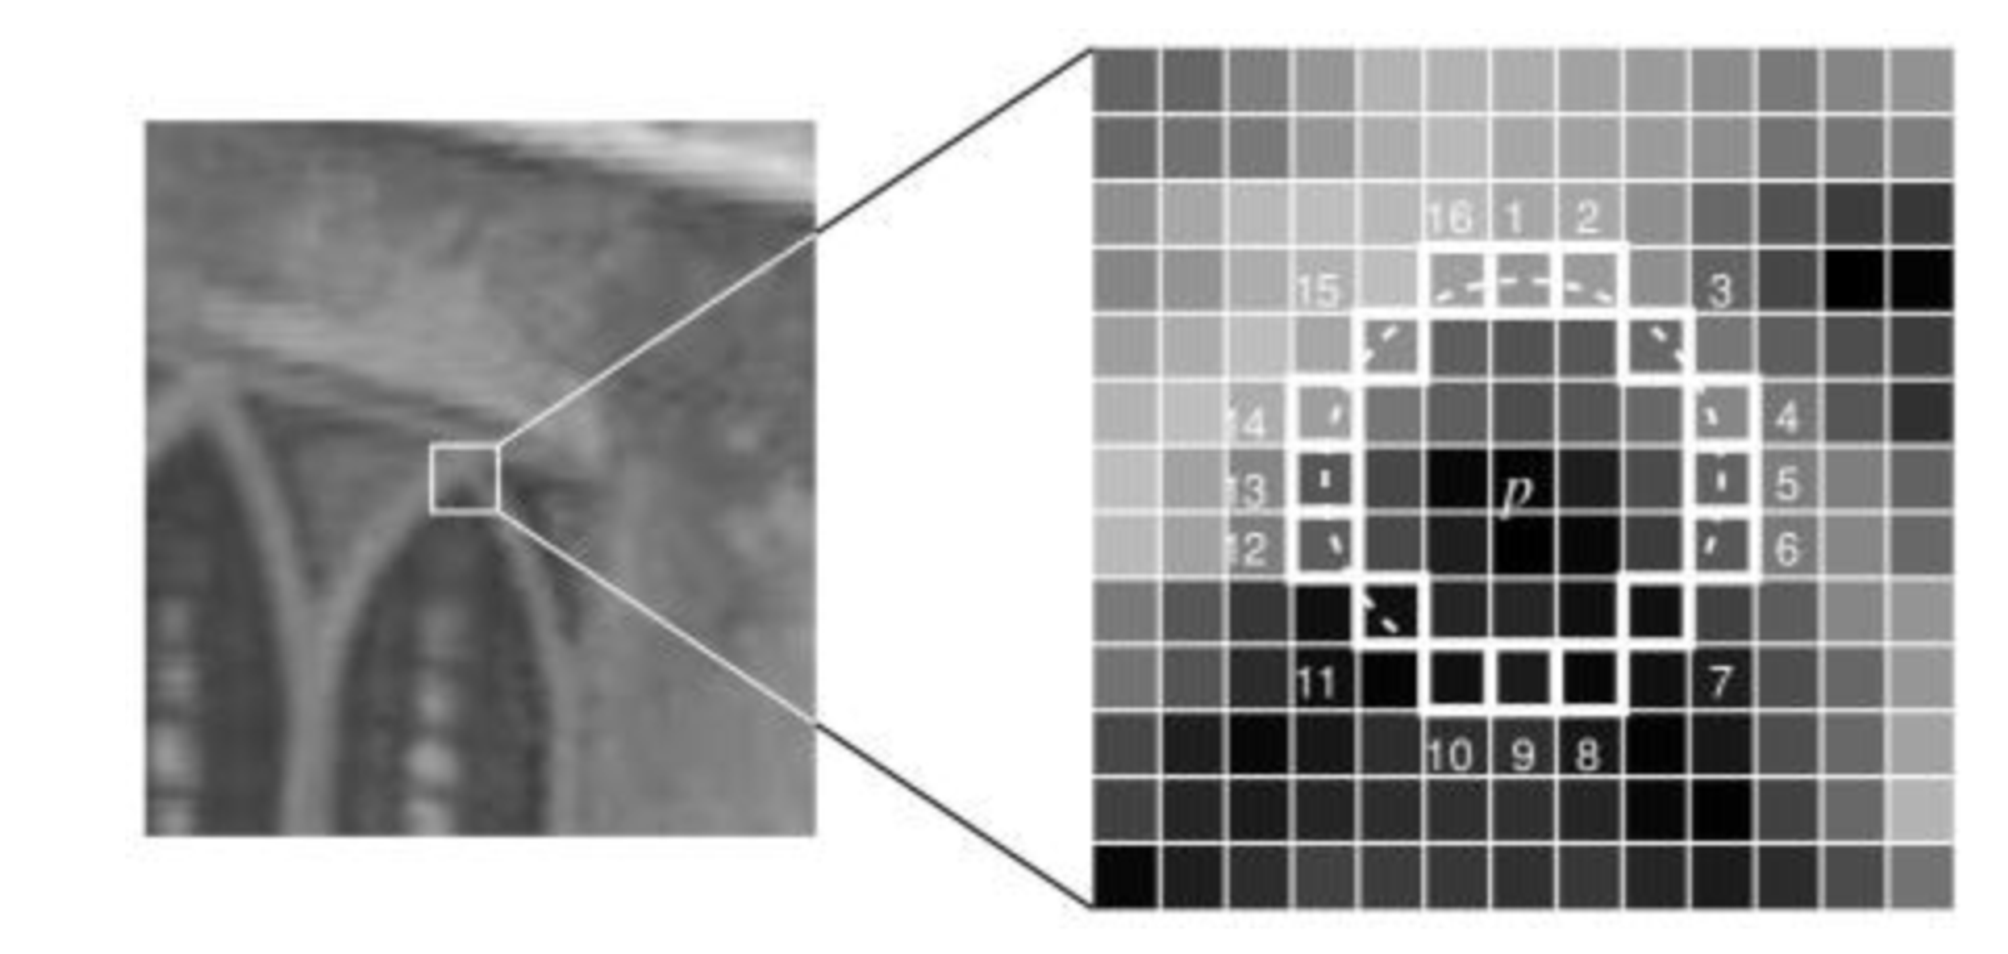
\includegraphics[width=120mm]{./figures/overview/fig1.eps}
    \end{center}
\end{figure}

\subsection{実装}
\begin{itemize}
    \setlength{\itemsep}{5mm}
    \item FASTの実装\par
    \vspace{1mm}
    \quad
    前節で述べたFASTの仕組みを以下のように実装した.
    なお,$t=50$,$n=12$とした.
    $n$の値は,FASTにおける高速化プログラムを意識した設定であるが,実験の結果,高速化のプログラムを織り交ぜた場合,ほとんどの試行に置いて,0.2sほどの遅れが見られたため,今回は高速化のプログラムを導入していない.
    \begin{enumerate}
        \item 画像をグレースケールに変換する.
        \item あるピクセルにおいて,その輝度値を$I_p$とする.
        また,周囲16ピクセルを抜き出し,その輝度値を配列に保存する.
        \item 2で抽出した16ピクセルについて,$I_p-t$より輝度が小さい,もしくは$I_p+t$より輝度が大きいピクセルの連続数を配列に格納する.
        ただし,最初と最後のピクセルで輝度条件が一致する場合は,最初の連続数と最後の連続数を足し合わせ,配列の末尾に格納する.
        \item 3で作った配列の要素の最大値を抽出し,その値が$n$以上であった場合,特徴点として認め,その座標を記録する.
        \item 2~5を画像中の「ほぼ」全てのピクセルに置いて繰り返す.(画像の端から10ピクセルに置いては処理をスキップする.これは後述するマッチング処理に置いて,エラーを防ぐためである.)
    \end{enumerate}
    \item 特徴点マッチングの実装\par
    \vspace{1mm}
    \quad
    特徴点のマッチングは以下のように行った.
    \begin{enumerate}
        \item 2つの画像について,特徴点を上記のFASTの実装を用いて特徴点抽出を行う.
        \item 各画像の特徴点周辺の10×10ピクセルを抜きだし,1次元化したのちに差分の絶対値を足し合わせる.
        これを「特徴点非類似度」として記録する.
        すなわち,この値が大きいほど特徴点は類似していないことになる.
        \item これを全ての特徴点組みに対して行い,「特徴点非類似度」がもっとも小さい2組をもっとも信頼のおける2組の特徴点対とし,変換行列を計算する.
    \end{enumerate}
\end{itemize}
